\documentclass{article}

\setlength{\parindent}{0pt} 

\usepackage{enumitem}
\usepackage{amsmath}
\usepackage{amssymb}
\usepackage{tikz}
\usetikzlibrary{automata, positioning}


\newlist{qanda}{enumerate}{1}
\setlist[qanda,1]{label=\textbf{Q\arabic*:}, 
                  left=0pt, 
                  itemsep=1em, 
                  align=left, 
                  wide=0pt}

\newcommand{\answer}[1]{\\\textbf{A:} #1}

\title{Theory of Computation}
\author{Mohammed Fahad}

\begin{document}

\maketitle

\section{Why TOC?}

\begin{itemize}
    \item It helps us to understand the limits of what computer can do and how to model computation using mathematics
\end{itemize}

\begin{qanda}
    \item What is the motivation for studying theory behind computation? OR Needs of TOC?
    \answer{
        \begin{itemize}
            \item Understanding the capability of a computer
            \item To find steps to solve a problem
            \item Increase efficiency while doing a task
        \end{itemize}
    }

    \item List the problems that cannot be solved by a computer.
    \answer{
        \begin{enumerate}
            \item Ethical problems. Eg: Self-driving car deciding to save the driver/passenger or the pedestrian
            \item Generating truly original art of emotion
        \end{enumerate}
    }

\end{qanda}

\section*{Automaton (pl.: Automata)}

A simplified mathematical model of a machine (digital computer). It 
\begin{itemize}
    \item Accepts input
    \item Produces output
    \item Nay have some temporary storage
    \item can make descisions in transforming the input into the output
\end{itemize}

\begin{qanda}
    \item Why study computability and theory?
    \answer{
        \begin{itemize}
            \item It helps to answer: "Can this be solved by a computer?"
            \item Understand the principles behind algorithms and programs
            \item Explore the boundary between what is possible and impossible in computing
        \end{itemize}
    }
\end{qanda}

\subsection{Need for mathematical modelling}
\begin{itemize}
    \item Computers work on rules \& logic
    \item We can represent computers using abstract models
    \item These models helps us study complex behaviour in a simplified way
\end{itemize}

\section{Introduction to finite automata}

\begin{enumerate}
    \item ON/OFF Switch:
        \begin{center}
        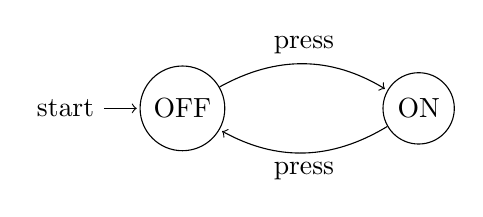
\begin{tikzpicture}[shorten >=1pt, node distance=3cm, on grid, auto]

        \node[state, initial] (OFF) {OFF};
        \node[state, right=of OFF] (ON) {ON};

        \path[->]
            (OFF) edge[bend left] node {press} (ON)
            (ON) edge[bend left] node {press} (OFF);

        \end{tikzpicture}
        \end{center}
    \item Coffee vending machine (Inputs: Rs. 5 \& Rs. 10 | Rs. 15 for one coffee):
        \begin{center}
        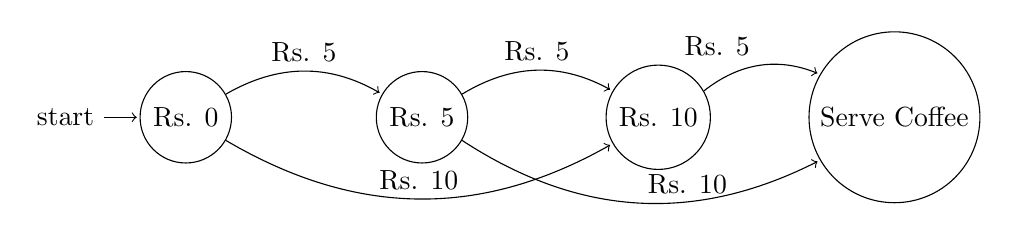
\begin{tikzpicture}[shorten >=1pt, node distance=3cm, on grid, auto]

        \node[state, initial] (NONE) {Rs. 0};
        \node[state, right=of NONE] (FIVE) {Rs. 5};
        \node[state, right=of FIVE] (TEN) {Rs. 10};
        \node[state, right=of TEN] (SERVE) {Serve Coffee};

        \path[->]
            (NONE) edge[bend left] node {Rs. 5} (FIVE)
            (FIVE) edge[bend left] node {Rs. 5} (TEN)
            (TEN) edge[bend left] node {Rs. 5} (SERVE)
            (NONE) edge[bend right] node {Rs. 10} (TEN)
            (FIVE) edge[bend right] node {Rs. 10} (SERVE);
        \end{tikzpicture}
        \end{center}

\end{enumerate}

\section{Formal Language}
A formal language is an abstraction of the general characteristics of programming langauges.

A formal language consists of set of symbols and some rules of formation by which these symbols can be combined into entities called sentences.

\section{Central concepts of automata theory}

\subsection{Alphabets}
It a finite, non-empty set of symbols. Alphabets are represented by '$\Sigma$'.

Binary alphabets can be represented as:
\[\Sigma = \{0, 1\} \]

Set of lowercase letters:
\[\Sigma = \{a, b, c, ... , z\} \]

\subsection{Strings}
A string is a finite seeunce of symbols chosen from some alphabets.

Eg:
Let $\Sigma = \{0, 1\}$ be the alphabet. \\

Examples of strings in $\Sigma$: 
\[
\ 0,\ 1,\ 00,\ 01,\ 10,\ 11,\ 000,\ 010,\ \ldots
\]

\subsubsection{Length of a string}
The number of occurances of symbols in the string.

\begin{align*}
\text{Length one:} \quad & 0,\ 1 \\
\text{Length two:} \quad & 00,\ 01,\ 10,\ 11
\end{align*}

The std. notation for length of a string $w$ is $\|w\|$

\subsubsection{Empty string ($\varepsilon$)}
A string with zero occurances OR string with length '0'

\subsubsection{$\Sigma^*$}
Set of all strings over an alphabet

\subsubsection{$\Sigma^+$}
Set of all strings excluding empty string over an alphabet
\[\Sigma^* = \Sigma^0 \cup \Sigma^+\]

\subsection{Powers of an alphabet}
If $\Sigma$ is an alphabet, $\Sigma^k$ is the set of strings with length 'k', each of whose symbols is in '$\Sigma$'.

\begin{align*}
    \Sigma^3 &= \{000,\ 001,\ 010,\ 011,\ 100,\ 101,\ 110,\ 111\} \\
    \Sigma^0 &= \{ \varepsilon \}
\end{align*}

NOTE: $\Sigma \neq \Sigma^1$, Their definitions differentiates them.

\section{Concatenation of strings}
Let $x$ and $y$ be strings, then $xy$ means combining both $x$ and $y$.

\begin{align*}
    &\text{i.e., if } x = 01010 \text{ and } y = 110, \\
    &xy = 01010110
\end{align*}

\begin{align*}
    &|x|=m \text{ and } |y| = n, \\
    &|xy| = m + n
\end{align*}

For any string $w$, then the equation,

\[ \varepsilon w = w \varepsilon = w \]

ie, $\varepsilon$ is the identity of Concatenation

\section{Languages}
A set of strings all of which are chosen from $\Sigma^*$. If $\Sigma$ is an alphabet, then $L \subset \Sigma^*$. Eg:

\begin{enumerate}
    \item Set of all strings consisting of $n$ 0s followed by $n$ 1s, $n \geq 0$
    \[
    L=\{\varepsilon, 01, 0011, 000111, ...\}
    \]
    \item Set of all strings having equal number of 0s and 1s,
    \[
    L=\{\varepsilon, 01, 0011, 0101, ...\}
    \]
\end{enumerate}

NB: $\Sigma^*$ is a language for any alphabet, $\Sigma$
\begin{align*}
    L = \{\} &\rightarrow \text{Empty language, } \varnothing \\
    L = \{\varepsilon\} &\rightarrow \text{Language containing the empty string}
\end{align*}

There are 2 types of Languages:
\begin{enumerate}
    \item \textbf{Infinte languages}. Eg: $\{0, 01, 001, 0001, 00001, ...\}$
    \item \textbf{Finte langauges}. Eg: $\{\varepsilon, a, b, ab, ba\}$
\end{enumerate}

\section{Set-formers as a way to define language}
\begin{equation*}
    \{w | w \text{ consists of equal number of 0s and 1st}\}
\end{equation*}

\section{Problems}
Problem is the question of deciding whether a given string is a member of some particular language.

\section{Automata}
An automaton is an abstract model of a digital computer.

\subsection{Key components of automata}
\begin{enumerate}
    \item Input file
    \item Control Ubit
    \item storage
    \item Output
\end{enumerate}

\subsection{Types of automata}
\begin{enumerate}
    \item Deterministic (DFA): One move per configuration (Predictable)
    \item Nondeterministic (NFA): Multiple possible moves
\end{enumerate}

Then there is automata like:
\begin{itemize}

    \item \textbf{Acceptor:} Says “yes” or “no” for an input.

    This simple automaton accepts the string `a`:
    \begin{center}
    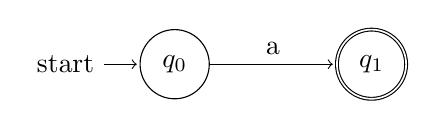
\begin{tikzpicture}[
      shorten >=1pt,
      node distance=2.5cm,
      on grid,
      auto
    ]
        \node[state, initial] (OFF) {$q_0$};
        \node[state, accepting, right=of OFF] (ON) {$q_1$};

        \path[->]
            (OFF) edge node {a} (ON);
    \end{tikzpicture}
    \end{center}

    \item \textbf{Transducer:} Produces an output string based on input.

    \begin{center}
        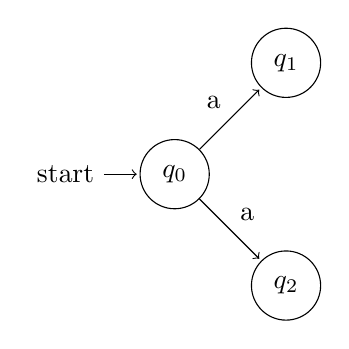
\begin{tikzpicture}[
        shorten >=1pt,
        node distance=2cm,
        on grid,
        auto
        ]
            \node[state, initial] (ONE) {$q_0$};
            \node[state, above right=of ONE] (TWO) {$q_1$};
            \node[state, below right=of ONE] (THREE) {$q_2$};

            \path[->]
                (ONE) edge node {a} (TWO)
                (ONE) edge node {a} (THREE);
        \end{tikzpicture}
    \end{center}

\end{itemize}

\end{document}
